%\documentstyle[11pt,a4]{article}
%\documentclass[a4paper]{article}
\documentclass[a4paper, 10pt]{article}
% Seems like it does not support 9pt and less. Anyways I should stick to 10pt.
%\documentclass[a4paper, 9pt]{article}
\topmargin-2.0cm

\usepackage{fancyhdr}
\usepackage{pagecounting}
\usepackage[dvips]{color}
\usepackage{wrapfig}
\usepackage{graphicx}

% Color Information from - http://www-h.eng.cam.ac.uk/help/tpl/textprocessing/latex_advanced/node13.html

% NEW COMMAND
% marginsize{left}{right}{top}{bottom}:
%\marginsize{3cm}{2cm}{1cm}{1cm}
%\marginsize{0.85in}{0.85in}{0.625in}{0.625in}

\def\ie{{\em i.e.,}}
\def\eg{{\em e.g.,}}
\newcommand{\tabref}[1]{Table~\ref{#1}}
\newcommand{\figref}[1]{Figure~\ref{#1}}
\newcommand{\secref}[1]{Section~\ref{#1}}

\advance\oddsidemargin-0.65in
%\advance\evensidemargin-1.5cm
\textheight9.2in
\textwidth6.75in
\newcommand\bb[1]{\mbox{\em #1}}
\def\baselinestretch{1.05}
%\pagestyle{empty}

\newcommand{\hsp}{\hspace*{\parindent}}
\definecolor{gray}{rgb}{0.4,0.4,0.4}
%\definecolor{gray}{rgb}{1.0,1.0,1.0}


\begin{document}
\thispagestyle{fancy}
%\pagenumbering{gobble}
%\fancyhead[location]{text} 
% Leave Left and Right Header empty.
\lhead{}
\rhead{}
%\rhead{\thepage}
\renewcommand{\headrulewidth}{0pt} 
\renewcommand{\footrulewidth}{0pt} 
\fancyfoot[C]{\footnotesize \textcolor{gray}{https://norouzi.github.io/}} 

%\pagestyle{myheadings}
%\markboth{Sundar Iyer}{Sundar Iyer}

\pagestyle{fancy}
\lhead{\textcolor{gray}{\it Mohammad Norouzi}}
\rhead{\textcolor{gray}{\thepage/\totalpages{}}}
%\rhead{\thepage}
%\renewcommand{\headrulewidth}{0pt} 
%\renewcommand{\footrulewidth}{0pt} 
%\fancyfoot[C]{\footnotesize http://www.stanford.edu/$\sim$sundaes/application} 
%\ref{TotPages}

% This kind of makes 10pt to 9 pt.
%\begin{small}

%\vspace*{0.1cm}
\begin{center}
{\LARGE \bf Research Statement}\\
\vspace*{0.1cm}
{\normalsize Mohammad Norouzi (mnorouzi@google.com)}
\vspace*{0.2cm}
\end{center}
%\vspace*{0.2cm}

%\begin{document}
%\centerline {\Large \bf Research Statement for Mohammad Norouzi}
%\vspace{0.5cm}

% Write about research interests...
%\footnotemark
%\footnotetext{Check This}


My research investigates the mathematical principles and modeling
assumptions that lead to the emergence of {\em Artificial Intelligence
  (AI)}.  I believe there exists a simple and universal algorithm that
can successfully address many different {\em Machine Learning (ML)}
problems. Hence, my research focuses on developing simple and generic
ML algorithms that are broadly applicable across a range of problem
domains including {\em computer vision}, {\em natural language
  processing}, and {\em sequential decision making}. I am interested
in bridging the gap between various existing ML paradigms
(\eg~see~\cite{raml,pcl}) to help simplify and unify common ML
objective functions and understand the benefits and weaknesses of each
approach. My research makes heavy use of {\em deep neural networks}
because of their flexibility and expressiveness
(\eg~\cite{seq2seq,alphago}) and intends to make neural nets even more
powerful and flexibl.esc

%% \begin{wrapfigure}{r}{2in}
%% %\begin{figure}
%% \vspace*{-.2cm}
%%   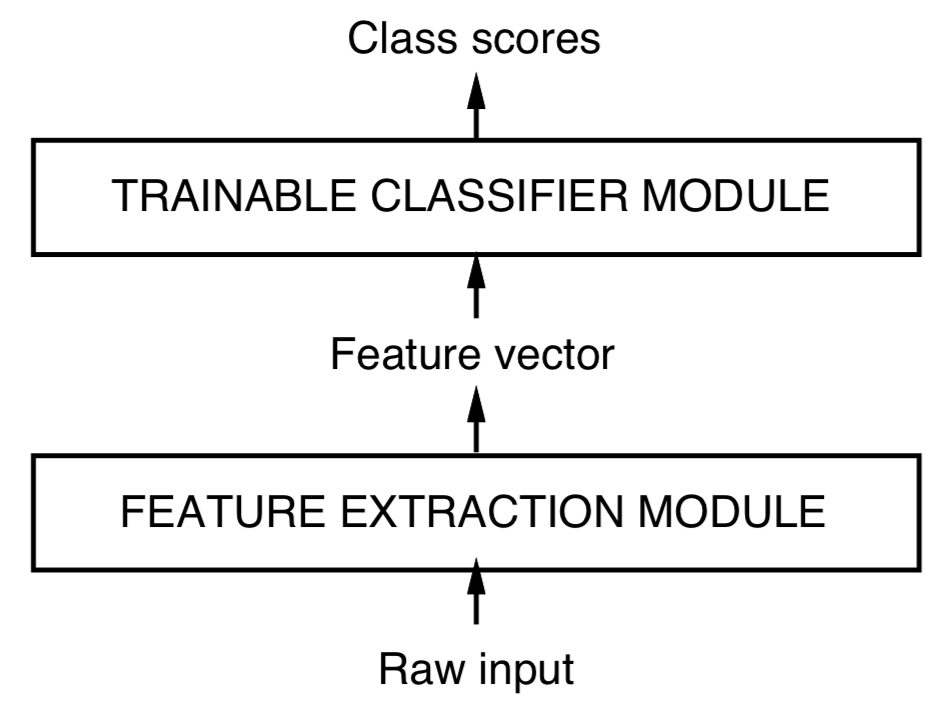
\includegraphics[width=2in]{fig1.png}
%% \vspace*{-.2cm}
%%   \caption{\small Figure from \cite{lecun98}, which highlights the
%%     inefficiency of traditional pattern recognition with separately
%%     tuned feature extraction and classification modules.}
%%   \label{fig:fig1}
%% \end{wrapfigure}

My current research aims to enable effective and efficient {\em
  end-to-end} optimization of multi-stage pipelines that involve {\em
  discrete} latent variables and {\em non-differentiable} components.
I am inspired by the success of error back propagation through
multilayer neural networks to jointly optimize hierarchical feature
extraction and classification modules~\cite{backprop,lecun98}.
%(\eg~\figref{fig:fig1}).
My research aspires to facilitate goal driven joint optimization of
complex AI systems, which comprise vision, natural language, memory,
and reasoning modules. I believe that by adopting an end-to-end
optimization approach, one can achieve higher degree of efficiency and
effectiveness in many hand-crafted pipelines.  For example, my
previous work has demonstrated the effectiveness of (1) end-to-end
optimization of metric learning and quantization
modules~\cite{mlh,hdml}, (2) non-greedy optimization of decision
trees~\cite{engodt}, (3) joint optimization of keypoint extraction and
pose estimation modules~\cite{keypointnet}, and (4) goal-driven
optimization of sequence models based on a sequence level reward
feedback~\cite{mapo,ocd}. Generally, end-to-end optimization results
in a big performance gain and offers a way to fine-tune separate
modules to encourage effective cooperation.

Discrete latent variables are ubiquitous in machine learning in
mixture models, efficient memory modules based on discrete codes,
models of hard attention~\cite{hardattention}, and structured output
prediction~\cite{}

Using discrete variables as intermediate ML
representations enables better {\em interpretability} and offers
valuable insights into the inner workings of ML systems. For example,
consider a question answering system that converts a natural language
question into an output answer. One can optimize a neural network to
directly map intput questions to output answers, or alternatively, a
neural network can first generate an intermediate SQL program, which
when executed on a database results in the final
answer~\cite{mapo}. Having access to an underlying latent program
allows one to understand the model's behavior and trace back an
incorrect answer to issues either in the database or in the model's
understanding of the question. Interpretability is especially
important for deploying ML systems in sensitive application areas such
as medicine and public policy. Nevertheless, end-to-end optimization
of discrete variables is often technically challenging due to lack of
differentiability.

\subsubsection*{Optimization of Discrete Variables via Reinforcement Learning Techniques}

To mitigate the non-differentiability of an objective function that
involves discrete latent variables, one can define a soft relaxation
of the original objective function in terms of

probability
distribution over latent variables and define the objective function
in terms of an expectation with resp

I draw inspiration from {\em
  Reinforcement Learning (RL)} and make use of stochastic
variablesadopt a stochastic smoothing of the discrete random
variables.

\subsubsection*{End-to-end Model-based Reinforcement Learning}
\subsubsection*{End-to-end Geometric Reasoning}


and define an stochastic variant of the
discrete variables.

\subsection{Memory}

My PhD research concerned with fast similarity search on large data
collections. I focused on distance metric learning and hashing as
important modules within a retrieval system. My main insight was that
these two modules should be optimized jointly to enable more efficiency.


I believe in order to build such intelligent systems,
one needs to facilitate {\em end-to-end} optimization of each module
jointly with other modules.



I de

I believe that a small
set of optimization functions can be used to optimize 


Can intelligent behavior be described using simple, elegant principles
(such as logic or optimization)? Or does it necessarily require
solving a large number of completely unrelated problems?[16]



My research lies at the intersection of machine learning algorithms
and applications in computer vision and natural language processing.
My current research aims to enable effective and efficient {\em
  end-to-end} optimization of complex multi-stage pipelines that
involve {\em discrete} latent variables and {\em non-differentiable}
components. 


My research lies at the intersection of machine learning algorithms
and applications in computer vision and natural language processing.
My current research aims to enable effective and efficient {\em
  end-to-end} optimization of complex multi-stage pipelines that
involve {\em discrete} latent variables and {\em non-differentiable}
components.  I am inspired by the success of error back propagation
through multilayer neural networks to jointly optimize hierarchical
feature extraction and classification modules. My research goal is to
facilitate goal driven joint optimization of big AI systems that
comprise computer vision, natural language, and sequential decision
making modules.

I am interested in developing simple and efficient machine learning
algorithms that result in emergence of intelligent behaviour 


, and effective machine learning
algorithms that are broadly applicable across a range of domains
including computer vision, natural language processing, and sequential
decision making. I aspire to help build artifical


My research aims to My research lies at the intersection of machine learning algorithms
and applications in computer vision and natural language processing.
My current research aims to enable effective and efficient {\em                                                                                            
  end-to-end} optimization of complex multi-stage pipelines that
involve {\em discrete} latent variables and {\em non-differentiable}
components.  I am inspired by the success of error back propagation
through multilayer neural networks to jointly optimize hierarchical
feature extraction and classification modules. My research aspires
to facilitate goal driven joint optimization of big AI systems that
comprise computer vision, natural language, and sequential decision
making modules. the mathetmatical foundation of intellignece.



I believe the underlying mathematical
foundations of inteligence  


 I believe there exists a class of generic and
simple models that can address problems in these seemingly different
domains.


My
current research focuses on {\em (1)} building generative models of
sequential data, sentences, programs, images, and other structured
objects.  {\em (2)} Advancing reinforcement learning algorithms and
applications. {\em (3)} Bridging the gap between sequence modeling,
imitation learning, and reinforcement learning to develop more
effective algorithms.


My current
research My research lies at the intersection of machine learning algorithms
and applications in computer vision and natural language processing.
My current research aims to enable effective and efficient {\em                                                                                            
  end-to-end} optimization of complex multi-stage pipelines that
involve {\em discrete} latent variables and {\em non-differentiable}
components.  I am inspired by the success of error back propagation
through multilayer neural networks to jointly optimize hierarchical
feature extraction and classification modules. My research aspires
to facilitate goal driven joint optimization of big AI systems that
comprise computer vision, natural language, and sequential decision
making modules.



My research lies at the intersection of machine learning algorithms
and applications in computer vision and natural language processing.
My current research aims to enable effective and efficient {\em                                                                                            
  end-to-end} optimization of complex multi-stage pipelines that
involve {\em discrete} latent variables and {\em non-differentiable}
components.  I am inspired by the success of error back propagation
through multilayer neural networks to jointly optimize hierarchical
feature extraction and classification modules. My research aspires
to facilitate goal driven joint optimization of big AI systems that
comprise computer vision, natural language, and sequential decision
making modules.

My research lies at the intersection of machine learning (ML)
algorithms and applications in computer vision and natural language
processing.  My current research aims to enable efficient and
effective {\em end-to-end} optimization of multi-stage ML pipelines
that involve {\em discrete} latent variables and {\em
  non-differentiable} components.  I am inspired by the success of
error back propagation through multilayer neural networks to jointly
optimize hierarchical feature extraction and classification modules.
%(see \figref{fig:fig1}).
My research aspires to facilitate similar
goal driven joint optimization of complex AI systems that comprise
various computer vision, natural language, and sequential decision
making modules.

Using discrete variables as intermediate ML representations can offer
valuable insights into the inner workings of ML systems, \ie~more {\bf
  interpretable} models. For example, consider a question answering
system that converts natural language questions to output
phrases. Such a model can either directly generate the output phrase
from the input question, or first generate an intermediate SQL program
that when executed on a database of facts results in an output
phrase. Having access to an underlying latent program allows one to
understand the system better and trace back an incorrect answer to
issues in the database or in the model's understanding of the
question. Interpretability is particularly important for deploying ML
systems in senstive areas such as medicine and public policy. That
said, end-to-end optimization of discrete variables is often
challenging due to lack of differentiability.

\subsubsection*{End-to-end Model-based Reinforcement Learning}
\subsubsection*{End-to-end Geometric Reasoning}

\subsection*{Network Architecture ---  A Research Agenda}

   In the course of my research, I have noticed that the overhead (in terms
of size, power and cost) of designing networking components, which give 
performance guarantees is small. 
This is mainly due to two reasons. First, the inherent nature of 
networking makes many of these problems tractable. Second, a number of
hardware advances in Architecture, insights in Algorithms {\it \&} Combinatorics, 
as well as analysis techniques from Probability, {\it \&} Queueing Theory 
aid in the design of elegant and simple solutions.
I envisage the field of {\it Network Architecture} created from the 
ground up, building upon the foundations of a number of fields
including those mentioned above.

%% IMP - Better examples rather than the old NAT, firewall are needed.
% Also need more newer examples.

In the near future, I am interested in the 
principles involved in the design of basic networking 
components. These include
hardware components (e.g. scalable memories, 
network processor and co-processor architectures) and 
software techniques (e.g. network algorithms, packet processing 
techniques). 
  Simultaneously, I intend to understand how large components, which use
the above building blocks can be architected.
My research will focus on how these basic and large
components can be built in a scalable manner while maintaining 
performance guarantees. 
In particular, examples of large components that I have a keen
interest in are switches 
(e.g. packet and circuit switches, multi-service routers etc.), 
security devices (e.g. firewalls and intrusion detection 
systems), network maintenance devices (e.g. measurement,
management infrastructure) and application aware devices
(e.g. web server load balancers, proxies) etc. 

% VIMP - Need to say why systems with performance guarantees can help in solving bigger problems.
% VIMP - How can we get "real" QOS? Solve "DOS" attacks?" etc.

 In the future, though performance and scalability will remain key,
I also intend to look at issues such as {\it fault tolerance, graceful degradation,
reliability and uptime} of networking systems, which will become more relevant. 
I also believe that as systems become increasingly large and 
inter-dependent, {\it simplicity in design and component 
re-use} will be major factors.
Parallelism can play a key role here.
%in aiding and abetting all of the above features. 
Indeed, many of our proposed solutions, involve component re-use and 
parallelism, which can aid and abet the above.

% Say something here about network wide phenomena, can we finally
% get multimedia streaming because of guarantees.

 My research will involve a good mix of futuristic and present 
day research. 
One part of my work will focus on fundamentally different proposals and
radical solutions. As an example
--- can we finally achieve real-time streaming over the Internet,
assuming that the various network components give performance guarantees?
In contrast, I intend to devote the other part of my work 
on practical systems, which have immediate relevance and impact in Industry.
I intend to work closely with a number of
researchers in related fields. Similarly, I intend to
collaborate with Industry in understanding and developing solutions
for practical problems. I believe my past experience of research
work done jointly with a number of colleagues as well as my prior record
of participation with Industry will help me achieve this. 
I am excited at the
prospect of learning, contributing, giving shape and making an
impact in this upcoming and challenging field.  


% IMP IMP - Staying ahead of Industry?? - MIT works like that...
% IMP IMP - Say something about research has a 2 pronged idea - Practical Significance and Staying ahead of
% the curve.
% aid and abet
% Say that simplicity is necessary to get reliability, availability...
% simpicity is helped by re-using components.
% Far Future.
%In the far future, I believe that our understanding of 
% Organization
% In the future the drive for parallelism will be governed by the design of fault tolerant systems.
% Scalability, Availability.
% I would like to work with Internet Researchers, 
% Collaborate in 
% Parallelism is meant also for fault tolerance.
% Most things in networking are evolutionary- happen and deployed slowly.
% Talk about how you are interested in industry influence also.
% Talk about Deflection Routing etc., other research.
% Growth of the field of network architecture.
% Parts of this field are seeing fruition.
% Nice to be in this field.
% Areas of queueing theory, probaility theory, algorithms, computer architecture
% Combinatorics are coming together.
% Far in the future.
% Interested in Industry impact and applications.

\vspace{0.5cm}
%\begin{flushright}
%Mohammad Norouzi
%\end{flushright}

%\end{small}
%\newpage

%\begin{thebibliography}{deSolaPITH}
% Change font size?
% \tiny, \footnotesize, \small,\normalsize, \large, \Large, \LARGE, and \huge 
%\begin{small}
\begin{footnotesize}

\bibliographystyle{plain}
\bibliography{bib.bib}

\end{footnotesize}

\end{document}

